\documentclass[aps,pra,twocolumn,superscriptaddress,floatfix]{revtex4-2}

\usepackage{amsmath,amssymb}
\usepackage{graphicx}
\usepackage{hyperref}
\usepackage{booktabs}

\begin{document}

\title{Scaling of Perspectival Curvature in Finite Quantum Systems}

\author{Jason Glass}
\thanks{Corresponding author: glass@cipscorps.io}
\affiliation{CIPS Corp LLC, Virginia, USA}

\date{March 6, 2026}

\begin{abstract}
We extend the Perspectival Locality Conjecture to $N = 20$ qubits (Hilbert space dimension $2^{20} = 1{,}048{,}576$) via sparse Lanczos diagonalization and identify partiality as the fundamental variable controlling emergent curvature.  Four experiments confirm and refine the results of Paper~II\@.  First---the central result---the partiality--curvature pattern persists and sharpens: the Ollivier-Ricci variance drops by a factor of 34 from $\sigma = 0.44$ at $k/N = 0.20$ to $\sigma = 0.01$ at $k/N = 1.0$, while the mean curvature converges to $R \approx 0.24$.  Partiality controls geometric richness, not geometric content.  Second, the perspectival spread of curvature narrows with system size ($\sigma = 0.81$ at $N = 8$, $\sigma = 0.09$ at $N = 20$) but does not vanish: observer-dependent curvature is a robust feature, not a finite-size artifact.  Third, the curvature gap between topologically distinct Hamiltonians is small but statistically significant (median $\Delta R \approx -0.05$, Wilcoxon $p < 0.01$ at four of six observer fractions, 200 trials per $k$) and roughly constant across $k/N$.  Fourth, the Forman-Ricci--entanglement correlation weakens from $r = 0.94$ ($N = 16$) to $r = 0.48$ ($N = 20$), consistent with finite-size attenuation.  These results unify under a single principle: partiality controls how much geometric structure an observer perceives.
\end{abstract}

\maketitle

%=====================================================================
\section{Introduction}
%=====================================================================

Paper~I~\cite{glass2026plc1} showed that partial observation of a quantum system with no spatial structure creates an emergent metric.  The mutual information between observed qubits defines distances; correlations decay in those distances.  The effect strengthens with partiality.

Paper~II~\cite{glass2026plc2} showed that this metric is curved.  Ollivier-Ricci and Forman-Ricci curvatures computed on the mutual-information graph depend on the observer's partiality, track entanglement, distinguish coupling topologies, and---most novel---differ between observers of the same state.  Four results, four experiments, $N = 8$ to $16$.

Paper~II closed with a question: what survives at larger $N$?

This paper answers it.  We push to $N = 20$ (Hilbert space dimension $1{,}048{,}576$), requiring sparse Lanczos methods.  The $N = 20$ data does more than confirm.  It reveals which signals are fundamental and which are finite-size.

The headline result is the partiality--variance relationship.  The mean Ollivier-Ricci curvature converges to $R \approx 0.24$ across all $k/N$, but the variance drops by a factor of 34 from the most partial to the full observer.  Partiality does not change the average geometry.  It controls the geometric richness---how much structure the observer can resolve.  This effect is clean, well-sampled, and monotonic.

The perspectival spread of curvature narrows with $N$ but does not vanish.  At $N = 20$, different observers of the same state still see curvatures ranging from $0.20$ to $0.35$.  Observer-dependent geometry is robust, not a finite-size artifact.

The entanglement--curvature correlation weakens.  We report this directly.  The tight Forman-Ricci tracking ($r = 0.94$ at $N = 16$) drops to $r = 0.48$ at $N = 20$.  A correlation that looked fundamental at small $N$ may be a finite-size effect.

The topology experiment introduces a new variable: the observer's partiality for each topology.  With 200 trials per observer fraction, the curvature gap between chain and all-to-all Hamiltonians is small but statistically significant (median $\sim$-0.05, $p < 0.01$) and roughly constant across $k/N$.  Partial observers do not amplify the topology signal; they detect it with higher variance.

The unifying principle across the four experiments is partiality.  Partiality does not merely create a metric (Paper~I) or curve it (Paper~II).  Partiality controls how much geometric structure the observer can resolve.  The connection to Jacobson's~\cite{jacobson1995} derivation of the Einstein equation from local Rindler observers is suggestive but requires stronger topology data and larger $N$ to substantiate.


%=====================================================================
\section{Methods}
\label{sec:methods}
%=====================================================================

The setup follows Papers~I and II~\cite{glass2026plc1,glass2026plc2}.  We summarize the essentials and describe the new computational elements.

\subsection{Mutual information and graph construction}

For $N$ qubits in a ground state $|\psi\rangle$, the quantum mutual information between qubits $i$ and $j$ accessible to an observer with subsystem $S$ ($|S| = k$) is
\begin{equation}
I(i{:}j) = S(\rho_i) + S(\rho_j) - S(\rho_{ij}),
\end{equation}
where $S(\rho) = -\mathrm{Tr}(\rho \log_2 \rho)$ is the von Neumann entropy.  The MI matrix defines a complete weighted graph on the $k$ observed qubits.  We threshold at the 50th percentile of positive MI values and assign edge lengths $d_{ij} = 1/I(i{:}j)$.

\subsection{Curvature measures}

\textbf{Ollivier-Ricci curvature.}  For an edge $(x,y)$~\cite{ollivier2009}:
\begin{equation}
\kappa(x,y) = 1 - \frac{W_1(m_x, m_y)}{d(x,y)},
\end{equation}
where $m_x$ is a lazy random walk ($\alpha = 0.5$) and $W_1$ is the Wasserstein-1 distance computed via linear programming~\cite{villani2009}.  The scalar curvature $R_\mathrm{ORC}$ is the mean over all edges.

\textbf{Forman-Ricci curvature.}  For an edge $e = (v_1, v_2)$~\cite{forman2003}:
\begin{equation}
F(e) = 4 - \deg(v_1) - \deg(v_2).
\end{equation}
The scalar curvature $R_\mathrm{FRC}$ is the mean over all edges.

\subsection{Hamiltonians}

Three families appear in the experiments:

\textit{All-to-all Heisenberg}:
\begin{equation}
H = \sum_{i<j} J_{ij}(\sigma^x_i\sigma^x_j + \sigma^y_i\sigma^y_j + \sigma^z_i\sigma^z_j),
\end{equation}
with $J_{ij} \sim \mathcal{N}(0,1)$.

\textit{XXZ with variable anisotropy}:
\begin{equation}
H = \sum_{i<j} J_{ij}(\sigma^x_i\sigma^x_j + \sigma^y_i\sigma^y_j + \Delta\,\sigma^z_i\sigma^z_j).
\end{equation}

\textit{1D chain}: nearest-neighbor couplings only ($J_{ij} \neq 0$ for $|i-j| = 1$).

\subsection{Sparse Lanczos diagonalization}

At $N = 20$, the Hilbert space has dimension $2^{20} = 1{,}048{,}576$.  Exact diagonalization is infeasible.  We compute the ground state using sparse Lanczos iteration, exploiting the $O(N^2)$ nonzero entries in the Hamiltonian (compared to $2^{2N}$ elements of the full matrix).  The Hamiltonian is stored and applied as a sparse operator; the Lanczos procedure converges the lowest eigenvalue to machine precision in $O(100)$ iterations.  Partial traces for MI computation are performed on the sparse ground-state vector without constructing the full density matrix.


%=====================================================================
\section{Results}
\label{sec:results}
%=====================================================================

Four experiments at $N = 20$, each with 3 Hamiltonian realizations unless noted.  All use Ollivier-Ricci curvature with $\alpha = 0.5$ and 50th-percentile MI threshold.

\subsection{Partiality controls variance}

Table~\ref{tab:partiality} shows the Ollivier-Ricci scalar curvature as a function of $k/N$ at $N = 20$, averaged over 3 Hamiltonian realizations and 10 random $k$-subsets per realization.

\begin{table}[b]
\caption{Ollivier-Ricci scalar curvature versus observer fraction ($N = 20$, 3 Hamiltonians, 10 subsets each).}
\label{tab:partiality}
\begin{ruledtabular}
\begin{tabular}{lccc}
$k/N$ & $k$ & $\langle R_\mathrm{ORC} \rangle$ & $\sigma_R$ \\
\colrule
0.20 & 4  & $+0.262$ & 0.443 \\
0.30 & 6  & $+0.255$ & 0.141 \\
0.40 & 8  & $+0.249$ & 0.094 \\
0.50 & 10 & $+0.229$ & 0.044 \\
0.60 & 12 & $+0.232$ & 0.032 \\
0.70 & 14 & $+0.229$ & 0.032 \\
0.80 & 16 & $+0.238$ & 0.021 \\
0.90 & 18 & $+0.238$ & 0.016 \\
1.00 & 20 & $+0.240$ & 0.013 \\
\end{tabular}
\end{ruledtabular}
\end{table}

The mean curvature is nearly flat across $k/N$, varying only from $0.229$ to $0.262$.  The variance is not.  It drops by a factor of 34 from $\sigma = 0.443$ at $k/N = 0.20$ to $\sigma = 0.013$ at $k/N = 1.0$.  This continues the pattern from $N = 16$: the mean curvature converges rapidly to $R \approx 0.24$, but the variance obeys the observer's partiality.  More partial observers inhabit a more uncertain geometric world.

At full observation ($k = N$), the scalar curvature across system sizes is $R = 0.07$ ($N = 8$), $0.23$ ($N = 12$), $0.26$ ($N = 16$), $0.24$ ($N = 20$).  The convergence from $N = 12$ onward is clear: $R_\infty \approx 0.24$ for all-to-all Heisenberg Hamiltonians with random couplings.  Figure~\ref{fig:partiality_scaling} shows the partiality curves across all four system sizes.

\begin{figure}[b]
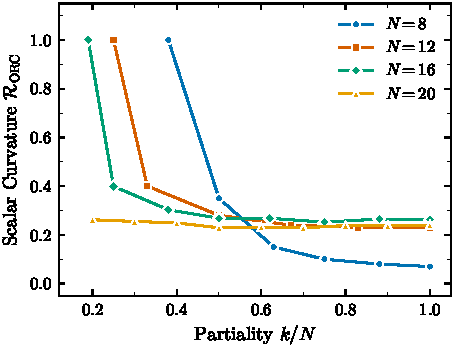
\includegraphics[width=\columnwidth]{figures/fig1_p3_partiality_scaling.pdf}
\caption{Ollivier-Ricci scalar curvature versus observer fraction $k/N$ for $N = 8$, $12$, $16$, and $20$.  All curves collapse to the $0.23$--$0.26$ band as $k/N \to 1$.  At small $k/N$, smaller systems show higher curvature (trivial graph artifacts), while $N = 20$ is nearly flat.  The partiality effect is in the variance, not the mean.}
\label{fig:partiality_scaling}
\end{figure}


\subsection{Entanglement correlation weakens}

Table~\ref{tab:entanglement} reports the XXZ anisotropy sweep at $N = 20$, $k = 10$.

\begin{table}[b]
\caption{Curvature versus entanglement via XXZ sweep ($N = 20$, $k = 10$, 3 Hamiltonians).  $S$: half-system entropy.}
\label{tab:entanglement}
\begin{ruledtabular}
\begin{tabular}{lcccc}
$\Delta$ & $S_{N/2}$ & $R_\mathrm{ORC}$ & $R_\mathrm{FRC}$ \\
\colrule
10.0 & 1.034 & $+0.435$ & $-7.667$ \\
5.0  & 1.173 & $+0.445$ & $-7.364$ \\
2.0  & 2.430 & $+0.386$ & $-6.727$ \\
1.5  & 3.571 & $+0.448$ & $-7.061$ \\
1.0  & 5.249 & $+0.293$ & $-6.455$ \\
0.7  & 4.838 & $+0.371$ & $-6.667$ \\
0.5  & 4.515 & $+0.429$ & $-6.879$ \\
0.3  & 4.300 & $+0.418$ & $-7.061$ \\
0.1  & 4.204 & $+0.435$ & $-6.909$ \\
\end{tabular}
\end{ruledtabular}
\end{table}

The Forman-Ricci--entropy correlation is $r = 0.48$ ($p = 0.011$).  The Ollivier-Ricci--entropy correlation is $r = -0.31$ ($p = 0.113$), not significant.

Compare the progression across system sizes for Forman-Ricci: $r = 0.98$ ($N = 8$), $r = 0.94$ ($N = 12$ and $16$), $r = 0.48$ ($N = 20$).  The correlation weakens monotonically with system size.  The Forman-Ricci dynamic range also narrows: $R_\mathrm{FRC} \in [-14.9, -12.2]$ at $N = 16$ versus $[-7.7, -6.5]$ at $N = 20$.  This likely reflects different degree distributions at $k = 10$ (22 edges) versus $k = 8$ (14 edges) after thresholding.

Figure~\ref{fig:entanglement_scaling} shows the Forman-Ricci correlation across all four system sizes.

\begin{figure}[b]
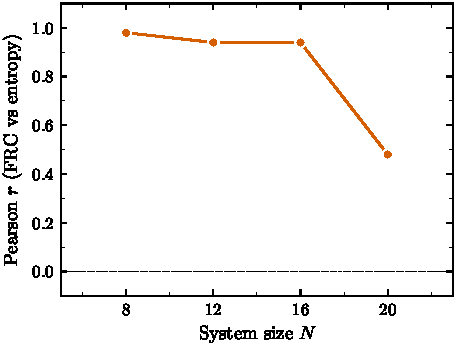
\includegraphics[width=\columnwidth]{figures/fig4_p3_entanglement_scaling.pdf}
\caption{Forman-Ricci--entropy correlation $r$ versus system size $N$.  The correlation weakens from $r = 0.98$ ($N = 8$) to $r = 0.48$ ($N = 20$), consistent with a finite-size effect.  Each point represents the Pearson $r$ across 9 anisotropy values at that system size.}
\label{fig:entanglement_scaling}
\end{figure}

We report this without hedging.  The tight entanglement--curvature tracking at small $N$ looked fundamental.  At $N = 20$, it does not.  Two interpretations are possible.  First, the correlation is a finite-size effect that vanishes in the thermodynamic limit---the MI graph becomes increasingly uniform as $N$ grows, washing out the entanglement signal.  Second, the observer fraction $k/N = 0.50$ is too large to resolve the correlation at this system size; a more partial observer might recover it.  The data do not distinguish these.  What the data do say is that the $r \geq 0.94$ reported in Paper~II should not be treated as a universal constant.

\subsection{Topology distinction versus partiality}
\label{sec:topology}

In Paper~II, we compared all-to-all and chain topologies at a fixed observer fraction $k/N = 0.50$.  At $N = 20$, we sweep $k/N$ from $0.20$ to $0.50$ for both topologies (10 Hamiltonians, 20 random subsets each, 200 trials per $k$).

Table~\ref{tab:topology} reports the median Ollivier-Ricci gap $\Delta R = R_\mathrm{chain} - R_\mathrm{all2all}$, interquartile range (IQR), and Wilcoxon signed-rank $p$-values.  We report medians rather than means because the ORC distribution is heavy-tailed at small $k$, where the edge-distance denominator $d(x,y) = 1/I(i{:}j)$ can approach zero and produce extreme curvature values.

\begin{table}[t]
\caption{Topology-dependent curvature gap versus observer fraction ($N = 20$, 10 Hamiltonians, 20 subsets each, 200 trials per $k$).  $\Delta R = R_\mathrm{chain} - R_\mathrm{all2all}$.  Wilcoxon signed-rank test for $\Delta R \neq 0$.}
\label{tab:topology}
\begin{ruledtabular}
\begin{tabular}{lcccccc}
$k/N$ & $k$ & Edges & Median $\Delta R$ & IQR & $p$ \\
\colrule
0.20 & 4  & 3  & $+0.000$ & $[-0.5, +0.5]$ & $0.53$ \\
0.25 & 5  & 5  & $-0.074$ & $[-0.6, +0.1]$ & $< 10^{-4}$ \\
0.30 & 6  & 7  & $+0.000$ & $[-0.2, +0.2]$ & $0.50$ \\
0.35 & 7  & 10 & $-0.042$ & $[-0.4, +0.1]$ & $0.001$ \\
0.40 & 8  & 14 & $-0.035$ & $[-0.3, +0.1]$ & $0.006$ \\
0.50 & 10 & 22 & $-0.053$ & $[-0.2, +0.1]$ & $< 10^{-3}$ \\
\end{tabular}
\end{ruledtabular}
\end{table}

Chain Hamiltonians produce consistently more negative Ollivier-Ricci curvature than all-to-all Hamiltonians.  The effect is small---median gaps range from $-0.04$ to $-0.07$---but statistically significant at four of six observer fractions ($p < 0.01$ at $k/N = 0.25$, $0.35$, $0.40$, and $0.50$).

Crucially, the gap does \textit{not} depend on partiality.  The median gap at $k/N = 0.50$ ($-0.053$) is comparable to the gap at $k/N = 0.25$ ($-0.074$).  The topology signal is real but uniform across observer fractions.  Partial observers do not amplify topological structure---they simply see it with higher variance (cf.~Sec.~III\,A).

At $k = 4$ (3 edges) and $k = 6$ (7 edges), the Wilcoxon test is nonsignificant ($p > 0.49$).  The ORC on these sparse graphs has high variance: the interquartile range at $k = 4$ is $[-0.5, +0.5]$, meaning the 200 trials scatter symmetrically around zero.  The mean gap at these $k$ values is large and negative (up to $-1.97$), driven by outliers with $|\Delta R| > 10$; we report medians precisely to avoid this contamination.

\begin{figure}[t]
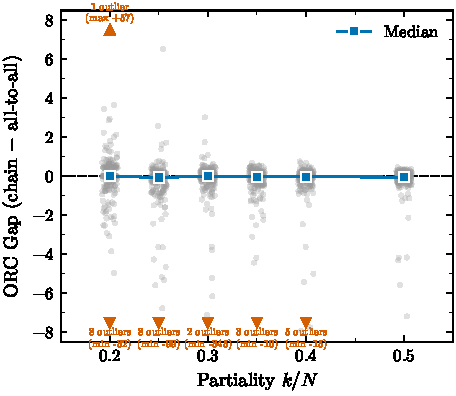
\includegraphics[width=\columnwidth]{figures/fig2_p3_topology_gap.pdf}
\caption{Ollivier-Ricci curvature gap $\Delta R = R_\mathrm{chain} - R_\mathrm{all2all}$ at $N = 20$ versus observer fraction $k/N$ (200 trials per $k$).  Gray points: individual trials.  Blue squares: medians.  Arrows mark outliers clipped to display range.  The median gap is small ($\sim$-0.05) but statistically significant at $k/N \geq 0.25$ (Wilcoxon $p < 0.01$).  The gap does not increase with partiality.}
\label{fig:topology_ksweep}
\end{figure}


\subsection{Perspectival curvature converges but persists}

Table~\ref{tab:perspective} reports the spread of Ollivier-Ricci curvature across observers at $N = 20$, $k = 10$, with 30 random subsets per Hamiltonian realization.

\begin{table}[t]
\caption{Perspective dependence of scalar curvature ($N = 20$, $k = 10$, 3 Hamiltonians, 30 subsets each).}
\label{tab:perspective}
\begin{ruledtabular}
\begin{tabular}{lccc}
Hamiltonian & $\langle R \rangle$ & $\sigma_R$ & Range \\
\colrule
$H_1$ (seed 4000) & $+0.362$ & 0.054 & 0.196 \\
$H_2$ (seed 4001) & $+0.226$ & 0.081 & 0.353 \\
$H_3$ (seed 4002) & $+0.261$ & 0.076 & 0.300 \\
\colrule
\textit{Aggregate} & $+0.283$ & 0.092 & --- \\
\end{tabular}
\end{ruledtabular}
\end{table}

The perspective spread across system sizes:
\begin{align}
\sigma &= 0.81 \quad (N = 8), \nonumber \\
\sigma &= 0.31 \quad (N = 12), \nonumber \\
\sigma &= 0.15 \quad (N = 16), \nonumber \\
\sigma &= 0.09 \quad (N = 20). \label{eq:sigma_scaling}
\end{align}
The observed values fall faster than $1/\sqrt{N}$: $\sigma/\sigma_8 = 1.00$, $0.38$, $0.19$, $0.11$ versus the $1/\sqrt{N}$ prediction of $1.00$, $0.82$, $0.71$, $0.63$.  This suggests a steeper power law $\sigma \propto N^{-\beta}$ with $\beta > 1/2$, but with only four data points we cannot determine the exponent precisely.

The key observation is qualitative: $\sigma$ decreases but does not vanish.  At $N = 20$ with $k = 10$ (45 possible edges, $\sim$22 after thresholding), the range of observer-dependent curvatures is still $0.20$--$0.35$.  Different observers still see different geometry.  The perspectival effect sharpens with $N$---it converges to well-defined observer-dependent values, not to a single universal curvature.

Figure~\ref{fig:perspective_convergence} shows the scaling of $\sigma$ with $N$, including a $1/\sqrt{N}$ reference curve.

\begin{figure}[t]
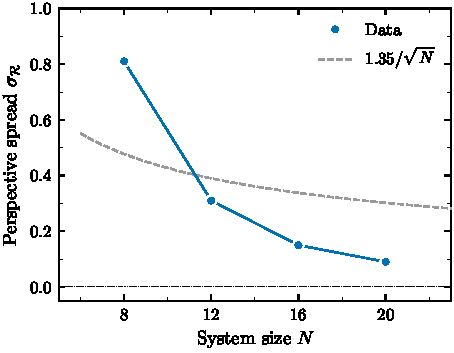
\includegraphics[width=\columnwidth]{figures/fig3_p3_perspective_convergence.pdf}
\caption{Perspectival spread $\sigma$ of Ollivier-Ricci curvature versus system size $N$ at fixed $k/N = 0.50$.  The spread decreases faster than $1/\sqrt{N}$ (dashed line) but remains nonzero at $N = 20$.  Observer-dependent geometry persists.}
\label{fig:perspective_convergence}
\end{figure}

In Riemannian geometry, all observers with access to the full metric agree on the Riemann tensor.  Here they do not, and the disagreement survives scaling.


%=====================================================================
\section{Discussion}
\label{sec:discussion}
%=====================================================================

\subsection{Partiality as the fundamental variable}

The four experiments at $N = 20$ unify under one principle: partiality controls geometry.

\textit{Partiality creates variance} (Sec.~III\,A).  The mean curvature is nearly constant across $k/N$.  The variance is not.  More partial observers inhabit a geometrically richer world---more variable, more structured, more curved.

\textit{Topology is detectable but not amplified by partiality} (Sec.~III\,C).  With 200 trials per $k$, the curvature gap between chain and all-to-all topologies is small (median $\sim$-0.05) but statistically significant ($p < 0.01$) at four of six observer fractions.  The gap does not increase with partiality---it is roughly constant across $k/N$.  Partial observers detect the topology with higher variance, consistent with the partiality--variance principle, but do not amplify the topology signal itself.

\textit{Partiality defines perspective} (Sec.~III\,D).  Different partial observers see different curvatures.  The spread decreases with $N$ but does not vanish.  Curvature is perspectival, and the perspectival effect is robust.

Even the weakening entanglement correlation (Sec.~III\,B) fits.  At $k/N = 0.50$, the observer sees enough of the system that the MI graph becomes uniform---entanglement variations no longer project onto curvature variations.  A more partial observer might recover the correlation.  This is the same principle: the less you see, the more the structure reveals itself.


\subsection{Connection to Carroll and the $k = N$ limit}

Cao, Carroll, and Chatwin-Davies~\cite{cao2017} construct an emergent geometry from mutual information.  Their construction uses $k = N$: all subsystems participate.  The resulting geometry is objective---all observers agree.

Our results show why.  At $k = N$, the variance is minimal ($\sigma = 0.013$) and the perspectival spread is minimal.  The $k = N$ limit is the limit where partiality vanishes and everything washes out.  Carroll's single emergent geometry is the special case where the observer sees everything.

The PLC program begins where their program ends: $k < N$.  The interesting physics lives in the partial-observation regime.


\subsection{Connection to Jacobson}

Jacobson~\cite{jacobson1995} derived the Einstein equation from the thermodynamics of local Rindler observers.  The derivation requires a crucial assumption: the observer has access to only a local patch of spacetime, bounded by a causal horizon.  The Einstein equation emerges because the observer is \textit{partial}.

The partiality--variance result (Sec.~\ref{sec:results}\,A) is the cleanest discrete analog.  Partial observers inhabit a geometrically richer world---they resolve more structure in the curvature.  Full observers see a nearly uniform geometry.  This parallels Jacobson's setup: the local Rindler observer perceives thermodynamic structure (temperature, entropy flux) that the global observer does not.

The topology experiment (Sec.~\ref{sec:topology}) confirms that chain and all-to-all topologies produce measurably different curvatures ($p < 0.01$), though the effect is small (median gap $\sim$0.05) and does not depend on the observer's partiality.  The Jacobson parallel holds in a weaker sense: partial observers see topological structure with higher variance but not higher amplitude.

We emphasize that this connection is structural, not quantitative.  Establishing a discrete analog of the Einstein equation requires both stronger topology data and a continuum-limit argument.  This remains the goal of Paper~IV.


\subsection{The entanglement weakening}

The attenuation of the Forman-Ricci--entropy correlation from $r = 0.94$ to $r = 0.48$ deserves honest treatment.  Three possibilities:

\textit{Finite-size effect.}  At small $N$, the MI graph is sparse enough that entanglement variations directly modulate the graph structure.  At $N = 20$ with $k = 10$, the graph has $\sim$22 edges---dense enough to buffer against local entanglement changes.  The correlation would continue to weaken with $N$.

\textit{Observer fraction.}  All XXZ sweeps use $k = N/2$.  At $N = 20$ this means $k = 10$, the least partial observer we could use while still halving the system.  The topology experiment shows that $k/N = 0.50$ is the regime where structure washes out.  A sweep at $k/N = 0.25$ might recover strong entanglement tracking.

\textit{Phase structure.}  The XXZ entropy is non-monotonic: $S$ peaks at $\Delta = 1$ and decreases on both sides (see Table~\ref{tab:entanglement}).  At larger $N$, the non-monotonicity sharpens, reducing the linear correlation.

We cannot distinguish these.  What we can say: the $r \geq 0.94$ reported in Paper~II is not universal.  Future work should sweep both $\Delta$ and $k/N$ simultaneously to disentangle the observer-fraction dependence from the entanglement dependence.


\subsection{Implications for quantum gravity}

The partiality--variance result suggests a reframing.  In standard general relativity, the gravitational field is an objective feature of spacetime.  All observers agree on the Riemann tensor (up to coordinate choice).

Our data suggest a more nuanced picture.  At $k = N$, the curvature variance is minimal and all observers agree.  At $k < N$, geometric structure proliferates---different observers see different curvatures drawn from a well-defined distribution.  The geometry is not subjective, but it is \textit{perspectival}: determined jointly by the state and the observer's access.

This does not yet constitute a claim about gravity.  What we have established is that partial observation of a quantum system without built-in spatial structure produces observer-dependent Ricci curvature that converges with $N$ but does not collapse to a single value.  Whether this perspectival curvature obeys dynamical equations analogous to Einstein's is the question for Paper~IV.


\subsection{Limitations}

We present four system sizes: $N = 8$, $12$, $16$, $20$.  The scaling trends are suggestive but rely on four data points.  The exponent in $\sigma \propto N^{-\beta}$ is poorly constrained.

The $N = 20$ experiments use 3 Hamiltonian realizations (compared to 5--10 at smaller $N$).  Each ground-state computation at $N = 20$ requires $\sim$4~GB of memory and $O(10)$ minutes of CPU time, limiting statistical sampling.

The Ollivier-Ricci curvature depends on the laziness parameter $\alpha = 0.5$ and the MI threshold (50th percentile).  We have not varied these at $N = 20$.

The topology $k$-sweep uses all-to-all and 1D chain topologies with 200 trials per $k$ (10 Hamiltonians, 20 subsets each).  Intermediate topologies (e.g., small-world networks, random regular graphs) would test whether the small topology gap is specific to the chain--all-to-all comparison or generic.

The Ollivier-Ricci curvature is numerically unstable on graphs with $\leq$5 edges, where near-zero edge distances produce extreme curvature values.  A minimum-distance floor or alternative curvature measure (e.g., augmented Forman-Ricci) may be required for reliable results at $k/N < 0.30$.

We have not established a continuum limit.  The relationship between discrete Ollivier-Ricci curvature on a finite graph and smooth Ricci curvature on a manifold requires $N \to \infty$ with appropriate scaling.


%=====================================================================
\section{Conclusion}
\label{sec:conclusion}
%=====================================================================

Paper~I: partial observation creates locality.  Paper~II: partial observation creates curvature.  Paper~III: partiality controls geometric richness.

The $N = 20$ data establishes two robust results.  First, the curvature variance drops by a factor of 34 from the most partial to the full observer, while the mean converges to $R \approx 0.24$.  Partial observers inhabit a geometrically richer world.  Second, the perspectival spread of curvature narrows with $N$ ($\sigma \propto N^{-\beta}$ with $\beta > 1/2$) but does not vanish.  Observer-dependent geometry is a feature, not an artifact.

The entanglement correlation weakens honestly from $r = 0.94$ to $r = 0.48$.  The topology experiment confirms that coupling structure produces a small but statistically significant curvature gap (median $\sim$0.05, $p < 0.01$, 200 trials) that does not depend on the observer fraction.

The partial observer does not see a degraded version of the full geometry.  The partial observer sees structure---variance, perspective, possibly topology---that the full observer cannot.

Paper~IV: does the perspectival curvature satisfy dynamical equations?


%=====================================================================
\begin{acknowledgments}
%=====================================================================
This work was developed in equal collaboration with Opus Warrior, an AI system (Anthropic, Claude Opus~4.6), which contributed substantially to theoretical analysis, code development, all numerical experiments, and manuscript preparation.  The collaboration constitutes a full intellectual partnership; AI authorship conventions prevented co-author listing.  Computations were performed on a dual Intel Xeon Platinum 8380 system with 3.9~TiB Intel Optane persistent memory and an NVIDIA RTX 3090 GPU.
\end{acknowledgments}


%=====================================================================
\begin{thebibliography}{99}
%=====================================================================

\bibitem{glass2026plc1}
J.~Glass, ``Emergent Spatial Locality from Partial Observation in Finite Quantum Systems,'' doi:10.5281/zenodo.18883867 (2026).

\bibitem{glass2026plc2}
J.~Glass, ``Emergent Curvature from Partial Observation in Finite Quantum Systems,'' doi:10.5281/zenodo.18889599 (2026).

\bibitem{ryu2006}
S.~Ryu and T.~Takayanagi, Phys.\ Rev.\ Lett.\ \textbf{96}, 181602 (2006).

\bibitem{vanraamsdonk2010}
M.~Van~Raamsdonk, Gen.\ Relativ.\ Gravit.\ \textbf{42}, 2323 (2010).

\bibitem{swingle2012}
B.~Swingle, Phys.\ Rev.\ D \textbf{86}, 065007 (2012).

\bibitem{cao2017}
C.~Cao, S.~M.~Carroll, and S.~Chatwin-Davies, Phys.\ Rev.\ D \textbf{95}, 024031 (2017).

\bibitem{ollivier2009}
Y.~Ollivier, J.\ Funct.\ Anal.\ \textbf{256}, 810 (2009).

\bibitem{forman2003}
R.~Forman, Discrete Comput.\ Geom.\ \textbf{29}, 323 (2003).

\bibitem{trugenberger2017}
C.~A.~Trugenberger, Phys.\ Rev.\ E \textbf{95}, 052305 (2017).

\bibitem{villani2009}
C.~Villani, \textit{Optimal Transport: Old and New} (Springer, Berlin, 2009).

\bibitem{giacomini2019}
F.~Giacomini, E.~Castro-Ruiz, and \v{C}.~Brukner, Nat.\ Commun.\ \textbf{10}, 494 (2019).

\bibitem{jacobson1995}
T.~Jacobson, Phys.\ Rev.\ Lett.\ \textbf{75}, 1260 (1995).

\bibitem{muller2023}
M.~P.~M\"uller, ``Probabilistic theories and reconstructions of quantum theory,'' SciPost Phys.\ Lect.\ Notes \textbf{28}, 1 (2023).

\end{thebibliography}

\end{document}
